\documentclass{../../Template}
\addbibresource{../../Bibliografia.bib} % si quieres incluir la bibliografía

\RequirePackage{transparent}


% Define el campo de subtitle como variable
\newcommand{\subtitle}[1]{\gdef\@subtitle{#1}}

\usetikzlibrary{fadings}

% Macro para hacer el título
\newcommand{\MakeTitle}[4]{%
\begin{titlepage} 

      %-----------------------------
      % --- CASO 0: MODO FOTO ----
      %-----------------------------

      \ifcase #1

      \begin{tikzpicture}[remember picture, overlay,x=\paperwidth, y=-\paperheight]
     
      % Fondo de color (opcional)
      \fill[#2] (current page.south west) rectangle (current page.north east);
      
      \node[opacity=1]  at (0.5,0.1) {\includegraphics[width=1.2\paperwidth]{#4}};

      % Sombra para autores
      \shade [opacity=0.3]
          (0.0, 0.23) rectangle (1.5, 0.35);
      \fill [opacity=0.2]
          (0.0, 0.23) rectangle (1.5, 0.35);

      \node [anchor=south west,align=left] at (0.05,0.32) {\fontsize{22pt}{24pt}\selectfont\bfseries \color{white} \theauthor\par};

      % Sombra para Titulo
      \shade [opacity=0.1,color = #2]
          (0.0, 0.35) rectangle (1.5,1.2);
      \fill [opacity=0.4,color = #2!10]
          (0.0, 0.35) rectangle (1.5,1.2);


      \node[anchor=north west,align=left,text width=0.9\paperwidth] at (0.05,0.38) {
        {\fontsize{60pt}{70pt}\selectfont \bfseries\color{white} \thetitle\par}
        \vspace{1em} \\[1 em]

        {\LARGE\itshape\color{white} \@subtitle\par}
        \vspace{3em}
      };

      % Lineas + Caja lado

      \fill [color=#2!50] (-0.2, 0.45) rectangle (-0.05, 0.36);

      
      \draw [ultra thick, opacity=0.8, color=white] (0.0,-1.5) -- (0.0,1.5);
      \draw [ultra thick, opacity=0.8, color=white] (-1.5,0.35) -- (1.5,0.35);
      
      \end{tikzpicture}

    
      
      %-----------------------------
      % --- CASO 2: MODO SIMPLE ----
      %-----------------------------

      \or 

      \begin{tikzpicture}[remember picture, overlay,x=\paperwidth, y=-\paperheight]
     
      
      % Fondo de color (opcional)
      \fill[#2] (current page.south west) rectangle (current page.north east);

      % Patron de color al fondo: 


      % Fondo (patron)

      % Sombra para autores
      \shade [ opacity=0.3, left color=#3, right color=#2]
          (0.0, 0.0) rectangle (1.5, 0.15);
      \node [anchor=north west,align=left] at (0.05,0.03) {\fontsize{22pt}{24pt}\selectfont\bfseries \color{white} \theauthor\par};

      % Sombra para Titulo
      \shade [opacity=0.4, left color=#3, right color=#2]
          (0.0, 0.15) rectangle (1.5,1.2);
          
      \fill [ opacity=0.3, color = #3]
          (-0.2, 0.15) rectangle (-0.01, 0.3);

      \node[anchor=north west,align=left,text width=0.9\paperwidth] at (0.05,0.18) {
        {\fontsize{56pt}{66pt}\selectfont \bfseries\color{white} \thetitle\par}
        \vspace{1em} \vspace*{2em}

        {\LARGE\itshape\color{white} \@subtitle\par}
        \vspace{3em}
      };
      \end{tikzpicture}
      
      %-----------------------------
      % --- CASO 3:            ----
      %-----------------------------

      \fi
      

    \null % Para evitar espacios verticales no deseados
    \thispagestyle{empty}
    \clearpage
  \end{titlepage}
}

% Para que \title y \author funcionen con \thetitle y \theauthor
\pretitle{\gdef\thetitle}
\preauthor{\gdef\theauthor}




%----------------------------------------------------------------------------
% ÍNDICE PERSONALIZADO
%----------------------------------------------------------------------------

\addto\captionsspanish{\renewcommand{\contentsname}{Índice general}}

\newlength{\fraseancho}
\newcommand{\hLinefill}[1]{\rule[0.5ex]{#1}{0.4pt}}

% Lo que se ejecutará al LEER el .toc
\DeclareRobustCommand{\TOCNewPart}[1]{%
  \par\begingroup
    \parindent=0pt
    \vspace{0.6\baselineskip}%
    \Large\bfseries
    \settowidth{\fraseancho}{#1}%
    \hLinefill{\dimexpr(0.95\linewidth-\fraseancho)/2\relax}%
    \hspace*{4mm}#1\hspace*{4mm}%
    \hLinefill{\dimexpr(0.95\linewidth-\fraseancho)/2\relax}%
    \par\vspace{0.3\baselineskip}%
  \endgroup
}

% Escribimos la llamada al macro anterior dentro del .toc
\newcommand{\NewPart}[1]{%
  \addtocontents{toc}{\protect\TOCNewPart{#1}}%
}

% Macro De Ejemplo

\RequirePackage[most]{tcolorbox}
\tcbuselibrary{skins}

\newcounter{Teorema}[chapter]
\newcounter{Definicion}[chapter]

%%%%%%%%%%%%%%%%%%%%%%%%%%%%%%%%%%%%%%%%%%%%%%%%%%%%%
% Ejercicio

\newcounter{exercise}[chapter]
\renewcommand{\theexercise}{\thechapter.\arabic{exercise}}

% Entorno Ejercicio
\newenvironment{Ejercicio}[1][]{%
  \refstepcounter{exercise}% <-- ancla de hyperref
  \begin{tcolorbox}[
  colback=Gray!40,
  colframe=Gray!40,
  sharp corners,
  boxrule=0pt,
  left=5pt,
  right=5pt,
  top=5pt,
  bottom=5pt,
  top=1.0em,          % margen superior interno (por encima del título y contenido)
  before title={\vspace{0.5em}}, % añade espacio encima del título
  %%
    title={\textcolor{black}{\bfseries \large Ejercicio~\theexercise}}, #1]%
}{%
  \end{tcolorbox}%
}

%%%%%%%%%%%%%%%%%%%%%%%%%%%%%%%%%%%%%%%%%%%%%%%%%%%%%%%
% Ejemplo

\newcounter{example}[chapter]
\renewcommand{\theexample}{\thechapter.\arabic{example}}

% Entorno Ejemplo

\newenvironment{Ejemplo}[1][]{%
  \refstepcounter{example}% <-- ancla de hyperref
  \begin{tcolorbox}[
  enhanced,         %
  colback=Gray!20,  %
  colframe=Gray!20, %
  sharp corners,    %
  left=5pt,         %
  right=5pt,        % 
  top=1.0em,        % margen superior interno (por encima del título y contenido)
  bottom=5pt,       %
  borderline south={3pt}{-3pt}{Gray}, % ← franja a la izquierda
  borderline north={3pt}{-3pt}{Gray}, % ← franja a la izquierda
  before title={\vspace{0.5em}}, % añade espacio encima del título
  title={\textcolor{black}{\bfseries Ejemplo~\theexample}}, #1]%
}{%
  \end{tcolorbox}%
}


%%%%%%%%%%%%%%%%%%%%%%%%%%%%%%%%%%%%%%%%%%%%%%%%%%%
% Teorema


\newcounter{theorem}[chapter]
\renewcommand{\thetheorem}{\thechapter.\arabic{theorem}}

% Entorno Teorema

\newenvironment{Teorema}[1][]{%
  \refstepcounter{theorem}% <-- ancla de hyperref
  \begin{tcolorbox}[
  enhanced,         %
  colback=Gray!30,  %
  colframe=Gray!30, %
  sharp corners,    %
  left=5pt,         %
  right=5pt,        % 
  top=1.0em,        % margen superior interno (por encima del título y contenido)
  bottom=5pt,       %
  borderline west={3pt}{-3pt}{Black!60}, % ← franja a la izquierda
  before title={\vspace{0.5em}}, % añade espacio encima del título
  title={\textcolor{black}{\bfseries Teorema~\thetheorem}}, #1]%
}{%
  \end{tcolorbox}%
}


%%%%%%%%%%%%%%%%%%%%%%%%%%%%%%%%%%%%%%%%%%%%%%%%%%%
% Definicion


\newcounter{definition}[chapter]
\renewcommand{\thedefinition}{\thechapter.\arabic{definition}}

% Entorno definicion

\newenvironment{Definicion}[1][]{%
  \refstepcounter{definition}% <-- ancla de hyperref
  \begin{tcolorbox}[
  enhanced,         %
  colback=Gray!20,  %
  colframe=Gray!20, %
  sharp corners,    %
  left=5pt,         %
  right=5pt,        % 
  top=1.0em,        % margen superior interno (por encima del título y contenido)
  bottom=5pt,       %
  borderline west={3pt}{-3pt}{Black!40}, % ← franja a la izquierda
  before title={\vspace{0.5em}}, % añade espacio encima del título
  title={\textcolor{black}{\bfseries Definición~\thedefinition}}, #1]%
}{%
  \end{tcolorbox}%
}



%%%%%%%%%%%%%%%%%%%%%%%%%%%%%%%%%%%%%%%%%%%%%%%%%%%
% Resalte


\newenvironment{Resalte}[1][]{%
  \begin{tcolorbox}[
  enhanced,         %
  colback=Gray!20,  %
  colframe=Gray!20, %
  sharp corners,    %
  left=5pt,         %
  right=5pt,        % 
  %left skip = 1cm,
  %rigth skip = 1 cm
  top=1.0em,        % margen superior interno (por encima del título y contenido)
  bottom=5pt,       %
  ]
}{%
  \end{tcolorbox}%
}

\lstdefinestyle{c++}{
  language=C++,                         % Base: C++
  numbers=none,        % Quita la numeración de líneas
  basicstyle=\footnotesize\ttfamily,
  numbers=left,
  numberstyle=\tiny,
  numbersep=5pt,
  stepnumber=1,
  tabsize=2,
  breaklines=true,
  frame=lines,
  xleftmargin=17pt,
  framexleftmargin=17pt,
  framexrightmargin=5pt,
  framexbottommargin=4pt,
  showspaces=false,
  showtabs=false,
  showstringspaces=false,
  stringstyle=\color{blue}\ttfamily,
  commentstyle=\color{green!50!black}\itshape,
  %
  % --- Core C++
  keywordstyle=\color{red}\bfseries,
  morekeywords={class,public,private,protected,namespace,using,
                new,delete,try,catch,throw,template,typename,
                sizeof,dynamic_cast,static_cast,const_cast,
                operator,this,virtual,override,final,constexpr},
  %
  % --- Tipos básicos
  keywordstyle=[2]\color{orange}\bfseries,
  morekeywords=[2]{int,double,float,char,bool,void,long,short,
                   string,auto,true,false,nullptr},
  %
  % --- ROOT (magenta)
  emph={TH1F,TH2F,TGraph,TCanvas,TF1,TTree,TChain,
        TFile,TBranch,TMath,TRandom,TRandom3,
        gROOT,gPad,gStyle,gApplication},
  emphstyle=\color{magenta}\bfseries,
  %
  % --- Geant4 (azul)
  emph={[2]G4RunManager,G4ParticleTable,G4ParticleDefinition,
        G4ThreeVector,G4RotationMatrix,G4Transform3D,
        G4VPhysicalVolume,G4LogicalVolume,G4Box,
        G4NistManager,G4Material,G4Element,
        G4PVPlacement,G4VSensitiveDetector,
        G4SystemOfUnits,G4UIcmdWithAString,G4UIcmdWithADouble},
  emphstyle=[2]\color{blue}\bfseries,
  %
  % --- Garfield++ (verde oscuro)
  emph={[3]MediumMagboltz,MediumSilicon,MediumGas,gas
        ComponentAnsys,ComponentElmer,ComponentAnalyticField,
        Sensor,ViewField,ViewCell,ViewDrift,
        AvalancheMicroscopic,AvalancheMC,TrackHeed},
  emphstyle=[3]\color{green!30!black}\bfseries,
  %
  % --- I/O (cian)
  emph={[4]cout,cin,endl,printf,sprintf,Form},
  emphstyle=[4]\color{cyan}\ttfamily
}


% Definiciones del título
\title{Simulación \ en \\ Física \ de \ Partículas}
\subtitle{Root, Geant4, CMake y Garfield++}
\author{Daniel Vázquez Lago}

% Documento

\begin{document}
\MakeTitle{1}{blue!80!black}{Snow1}


\setlength{\parskip}{2.4mm} % Cambia el espacio entre párrafos

\newpage

\tableofcontents

\chapter{Instalación, configuración y ejecucción de archivos}

\section{Instalación}

\subsection{Linux}

\section{Ejecucción de ejemplo}


\section{Configuración de VSCode}
\chapter{Garfield++}


\section{Introducción}

\textbf{Garfield++} es una herramienta basada en la programación orientada a objetos que permite simulaciones detalladas de detectores de partículas basadas en ionización de gases o semiconductores. Para calcular los campos eléctricos, se ofrecen ls siguientes técnicas: 

\begin{itemize}
    \item Soluciones para hilos/cables finos para detectores basados en hilos y planos. 
    \item Interfaces\footnote{Conexión funcional entre dos sistemas, programas, dispositivos o componentes de cualquier tipo, que proporciona una comunicación de distintos niveles, permitiendo el intercambio de información.} para elementos finitos, que pueden calcular campos aproximados en configuraciones 2 y 3 dimensionales con materiales dieléctricos y conductores. 
\end{itemize}
Para calcular las propiedades de tranpsorte de las partículas en mezclas de gases, usamos la interfaz de Magboltz. La ionización producida por partículas cargadas relativistas se estudia a través del programa Heed. Para la simulación de ionización producida por iones a baja energía, los resultados puede ser estudiado por el paquete SRIM. El programa Degrade simula la ionizacion producida por electrones. 

Un resumen de Garfield, o de un programa de Garfield, sería el siguiente:

\begin{enumerate}
    \item Primero tenemos que describir el medio (gas, silicio), información almacenada en un objeto clase \texttt{Medium}.
    \item Luego tenemo que definir el campo eléctrico en toda la región de interés. Existen varias maneras de definir el campo, en general se hace a través de la clase \texttt{Component}, en alguna de sus diferentes variantes. Por ejemplo puede ser importada a través de documentos externos, definido para geometrías sencillas por programas propios de Garfield++, o incluso definido por el usuario a mano. 
    \item También está la clase \texttt{Sensor}, que se encarga de definir el detector de las partículas cargadas. 
    \item Una vez hemos creado el sistema, el detector propiamente dicho, pasamos a la parte de ionización. Lo primero es crear la clase \texttt{Track}, que se encarga vía diferentes modelos (Heed, SRIM, Degrad) de crear los cluster de partículas productos de la ionización. En función de la partícula habrá que aplicar un modelo u otro (en el caso de iones pesados SRIM o TRIM, para otros Degrad o Heed). En casos extremos debemos enlazar Geant4 y Garfield++.
    \item Una vez se han creado los diferentes clusters, podemos simular su movimiento hacia los sensores (en el campo eléctrico) a través de la clase \texttt{Drift} para varios modelos (Runge-Kutta-Fehlberg, Montecarlo, Seguimiento Micorscópico). 
    \item Una vez llega al sensor se puede visualizar la señal. 
\end{enumerate}



\begin{Ejemplo}{\textbf{Tubo de deriva}}

En est ejemplo vamos a considerar un tubo de deriva con un diámetro de 15 mm y un diámetro del hilo (cable) de 50 $\mu m$, similar a los tubos de derivas de muones del ATLAS (también con un diámetro pequeño) llamados sMDTs. Primero importamos los módulos: \\

\begin{lstlisting}[language=C++,style=c++]
#include "Garfield/MediumMagboltz.hh"
#include "Garfield/ViewMedium.hh"
\end{lstlisting}

\vspace*{1em}


Lo primero que tenemos que hacer es preparar la \textbf{tabla de gases}, es decir, la tabla que contiene los parámetros de transporte (velocidad de deriva, coeficientes de difusión, coeficiente de Townsend, coeficiente de captura) como funciones del campo eléctrico $\Encal$ (y en general, del campo magnético $\Bn$ y el ángulo entre $\Encal$ y $\Bn$) para un gas a una temperatura y presión determinadas. En este ejemplo usaremos un gaz mezcla, a 3 atm y temperatura ambiente: \\

\begin{lstlisting}[language=C++,style=c++]
MediumMagboltz gas("ar", 93., "co2", 7);
// Set temperature [K] and preasure [Torr]
gas.SetPressure(3*760.);
gas.SetTemperature(293.15);
\end{lstlisting}

\vspace*{1em}

También debemos especificar el número de puntos de la malla campo eléctrico que vamos a usar en la tabla y el rango que va a ser cubierto. Usamos 20 puntos entre 100 V/cm a 100 kV/cm con un espaciado logaritmico:   \\

\begin{lstlisting}[language=C++,style=c++]
gas.SetFieldGrid(100.,100.e3,20,true);
\end{lstlisting}

\vspace*{1em}
    
Ahora ejecutamos Magboltz para generar una tabla del gas para esta malla de campo eléctrico. Como un parámetro de entrada tenemos que especificar \textit{el número de colisiones} (en múltiplos de $10^7$) sobre el electrón cuya traza dibuja Magboltz: \\

\begin{lstlisting}[language=C++,style=c++]
const int ncolll=10;
\end{lstlisting} 

Aunque tarde un rato, una vez este acabado podemos guardar los parámetros:  \\

\begin{lstlisting}[language=C++,style=c++]
gas.WriteGasFile("ar_93_co2_7.gas");
\end{lstlisting} 

\vspace*{1em}

para luego poder importarlos cuando queramos, y no tener la necesidad de correr el programa cada vez que los queramos: \\


\begin{lstlisting}[language=C++,style=c++]
gas.LoadGasFile("ar_93_co2_7.gas");
\end{lstlisting} 

\vspace*{1em}

Una buena idea podría ser, para asegurarse que el cálculo es correcto, graficar la velocidad de deriva en función del campo eléctrico: \\

\begin{lstlisting}[language=C++,style=c++]
ViewMedium view;
view.SetMedium(&gas);

// Dibujamos: 
TCanvas* c1 = new TCanvas("c1", "Propiedades del gas", 800, 600);
view.PlotElectronVelocity();
c1->SaveAs("drift_velocity.pdf");
\end{lstlisting} 

\begin{center}
    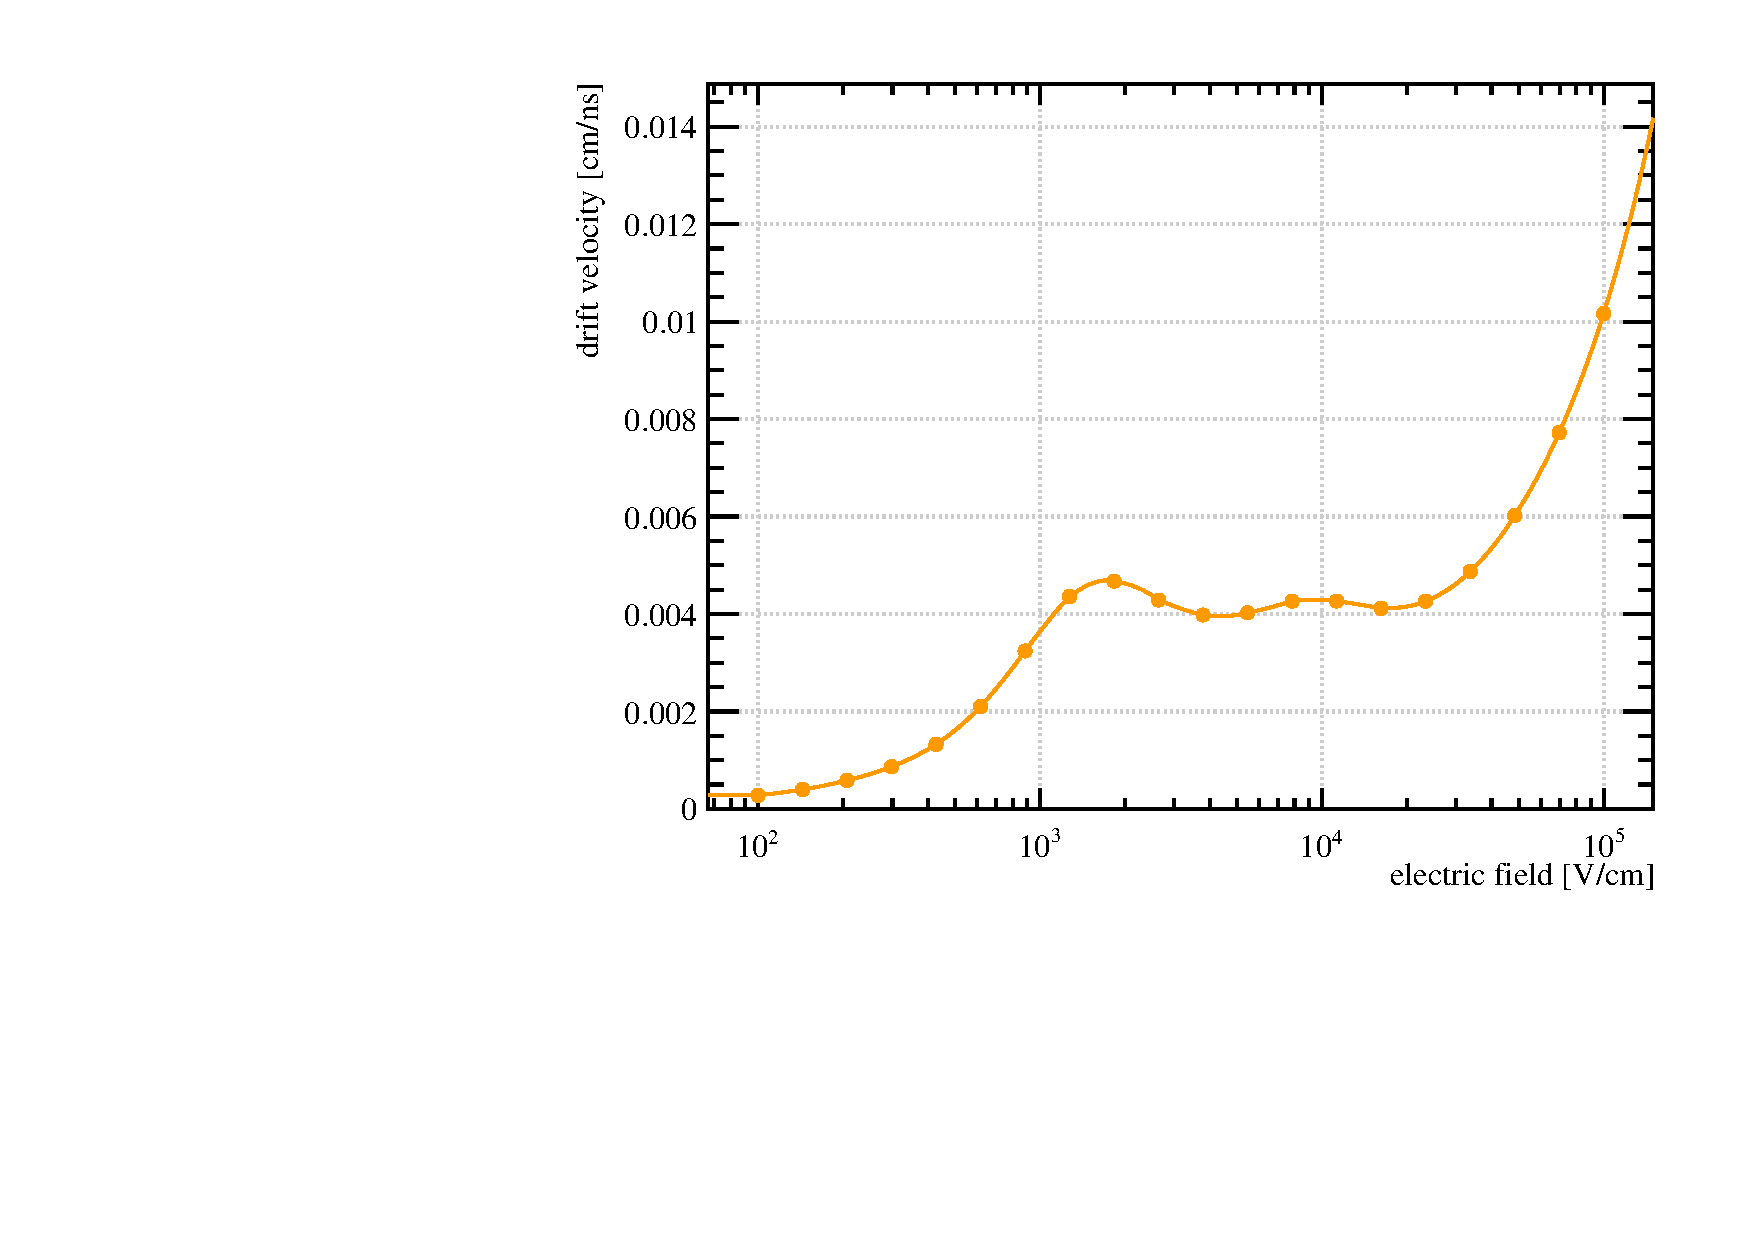
\includegraphics[width=0.6\linewidth]{Chapters/EjemploGarfield/TuboDeriva/build/drift_velocity.pdf}
\end{center}

Ahora podemos calcular el  \textbf{campo eléctrico} que se hace a través de \texttt{ComponentAnalyticField}, que básicamente maneja la disposición de cables, planos y tubos: \\

\begin{lstlisting}[language=C++,style=c++]
ComponentAnalyticField cmp;
\end{lstlisting} 

\vspace*{1em}

Tenemos que introducir el medio que hemos definido en la región activa: \\

\begin{lstlisting}[language=C++,style=c++]
cmp.SetMedium(&gas);
\end{lstlisting} 

\vspace*{1em}

Lo siguiente que tenemos que hacer es añadir los elementos que definen el campo eléctrico, i.e. el cable (denominado ``s'') y el tubo: \\


\begin{lstlisting}[language=C++,style=c++]
// Radio del cable [cm]
const double rWire = 25.e-4;

// Radio del tubo externo [cm]
const double rTube = 0.71;

// Voltajes 
const double vWire = 2730.;
const double vTube =    0.;

// Añadimos el cable en el centro de la disposición 
cmp.Addwire(0,0,2 * rWire, vWire, "s");

// Añadimos el tubo
cmp.AddTube(rTube, vTube, 0);
\end{lstlisting} 
\vspace*{1em}

Finalmente, creamos un \texttt{Sensor}, que es un objeto que actúa como interfaz en la clase transporte  discutido más abajo: \\


\begin{lstlisting}[language=C++,style=c++]
// Calculamos el campo eléctrico usando el objeto Componente cmp.
Sensor sensor(&cmp);
// Hacemos una petición para que calcule la señal del electrodo llamado s
//     usando el campo dado por el objeto Componente cmp.
sensor.AddElectrode(&cmp,"s");
\end{lstlisting} 
\vspace*{1em}

Ahora necesitadmos definir el intervalo temporal en el que la señal es guardada y la granularidad (ancho del bin). Podemos usar 1000 bins con un ancho de 0.5 ns \\

\begin{lstlisting}[language=C++,style=c++]
const double tstep = 0.5;
const double tmin = -0.5 * tstep;
const unsigned int nbins = 1000;
sensor.SetTimeWindow(tmin,tstep,nbins);
\end{lstlisting} 
\vspace*{1em}

Ahora lo que nos queda es \textbf{simular la ionización producida} por la partícula en el tubo de carga usando Heed, de un muón, con por ejemplo, 170 GeV. \textit{Track} significa camino o trayectoria en ingles. \\

\begin{lstlisting}[language=C++,style=c++]
TrackHeed track(&sensor);
track.SetParticle("muon");
track.SetEnergy(170.e9);
\end{lstlisting} 
\vspace*{1em}

Las curvas (lineas) de deriva de los electrones se crean usando el método de integración Runge-Kutta:fehlberg (RKF), implementada en la clase \texttt{DriftLineRKF}. Este método usa las tablas previamente computadas de parámetros de transporte para calcular las líneas de deriva y su multiplicación: \\


\begin{lstlisting}[language=C++,style=c++]
DriftLineRKF drift(&sensor);
\end{lstlisting} 
\vspace*{1em}

Consideremos ahora que la pista pasa a una distancia de 3 mm del centro del hilo. Después de simular el paso de la partícula cargada, nos tenemos que fijar en los ``clusters'' (agrupaciones de partículas cargadas producidas por la partícula primaria) y su movimiento en el dispositivo. Así pues, calculamos las líneas de deriva para cada electrón producido en el cluster: 

\begin{lstlisting}[language=C++,style=c++]
const double rTrack = 0.3;
const double x0=rTrack;
const double y0 = -sqrt(rTube * rTube - rTrack * rTrack)
track.NewTrack(x0,y0,0,0,0,1,0);
// Hacemos un bucle sobre los clusters producidos por el camino (track)
for (const auto& cluster: track.GetClusters()) {
    // Bucle alrededor de los electrones del cluster
    for (const auto& electron: cluster.electrons) {
        drift.DriftElectron(electron.x,electron.y,electron.z,electron.t)
    }
}
\end{lstlisting} 
\vspace*{1em}

Como una comprobación de la simulación podemos visualizar las líneas de deriva. Antes de simular el recorrido de la partícula cargada y las curvas de deriva de los electrones, tenemso que decirle a \texttt{TrackHeed} y \texttt{DriftLineRKF} que pase las coordenadas de los clusters y los puntos de las líenas de deriva al objeto \texttt{ViewDrift}, que se encarga de graficarlas:  \\

\begin{lstlisting}[language=C++,style=c++]
// Creamos un canvas
cD = new TCanvas ("cD"," ", 600, 600);
ViewDrift driftView;
drift.EnablePlotting(&driftView);
track.EnablePlotting(&driftView);
cellView.SetCanvas(cD);
cellView.Plot2d();
constexpr bool twod=true;
constexpr bool drawaxis = false;
driftView.Plot(twod,drawaxis);
cD->SaveAs("drift_view.pdf");
delete cD;
\end{lstlisting} 
\vspace*{1em}
Podemos graficar la señal inducida en el hilo/cable por la deriva de los electrones simulados:  \\

\begin{lstlisting}[language=C++,style=c++]
TCanvas* cS = new TCanvas("cS","",600,600);
sensor.PlotSignal("s",cS);
\end{lstlisting} 
\vspace*{1em}

\begin{center}
    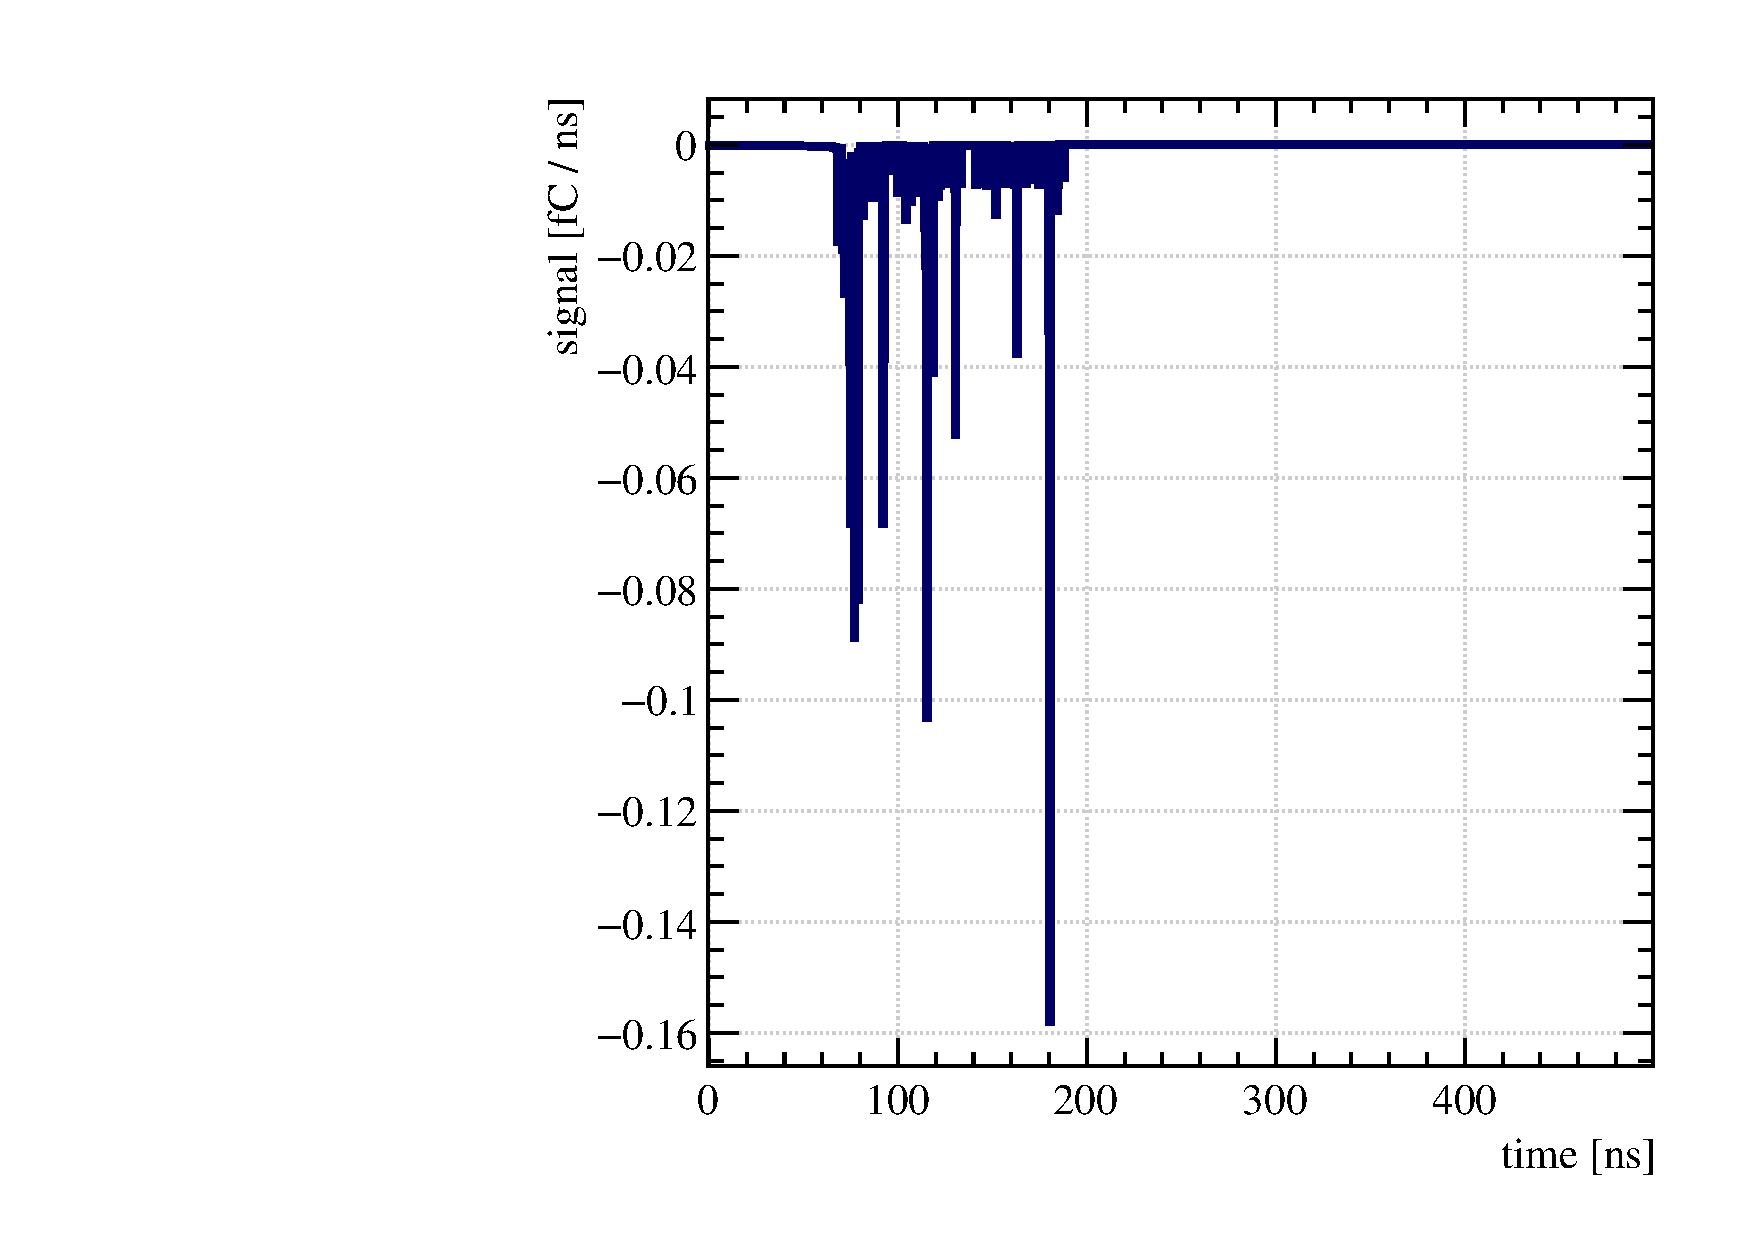
\includegraphics[width=0.6\linewidth]{Chapters/EjemploGarfield/TuboDeriva/build/signal.pdf}
\end{center}

Si quisieramos considerar la contribución de los iones producidos en la avalancha necesitamos importar tablas de mobilidades de iones: \\


\begin{lstlisting}[language=C++,style=c++]
gas.LoadIonMobility("LoadIonMobility_Ar+_Ar.txt")
\end{lstlisting} 
\vspace*{1em}

que, por defecto, \texttt{DriftLineRKF} las incluirá en la simulación. 






\end{Ejemplo}

\section{Medio}

La clase \texttt{Medium} incorpora las propiedades del medio. 

\begin{itemize}
    \item El \textbf{coeficiente Townsend} $\alpha$ nos habla de cuantos pares de iones se generan por unidad de longitud para una partícula cargada en movimiento, tal que:
    \begin{equation}
        I = I_0 e^{\alpha d}
    \end{equation}
    siendo $I$ la intensidad de corriente que circula por el dispositivo, $I_0$ la intensidad de corriente generada por efecto fotoeléctrico en el cátodo y $d$ la distancia entre cátodo y ánodo.
    \item El \textbf{coeficiente de captura} o \textit{attachment coefficient} nos habla de cuantos electrones/iones son capturados por el medio.
\end{itemize}

\subsection{Parámetros de transporte}

La clase \texttt{Medium} provee al usuario de las siguientes funciones para el cálculo de los parámetros de transporte de los electrones en función del campo eléctrico y magnético. 

\subsubsection{Visualización}

Los parámtros de transporte se pueden graficar en función del campo eléctrico a través de: \\

\begin{lstlisting}[language=C++,style=c++]
void PlotVelocity(const std::string& carriers, TPad* pad);
void PlotDiffusion(const std::string& carriers, TPad* pad);
void PlotTownsend(const std::string& carriers, TPad* pad);
void PlotAttachment(const std::string& carriers, TPad* pad);
void PlotAlphaEta(const std::string& carriers, TPad* pad);
\end{lstlisting}

\vspace*{0.7em}

donde la opción \texttt{carriers} indica la partícula cargada (ej: \texttt{''e''} indicaría electrones) para el cual vamos a garficar los parámetros.  Por ejenmplo para visualizar las líneas de velocidad de deriva electrónica y de huecos en silicio así como el coeficiente Townsend y de captura: \\

\begin{lstlisting}[language=C++,style=c++]
MediumSilicon si;
TCanvas* c1 = new TCanvas("c1", "", 600, 600);
si.PlotVelocity("eh", c1);
TCanvas* c2 = new TCanvas("c2", "", 600, 600);
si.PlotAlphaEta("eh", c2);
\end{lstlisting}

\vspace*{0.7em}

\subsection{Gases}

Hay dos clases principales implementadas que se pueden usar para la descripción de medios gaseosos. La primera sería \texttt{MediumGas} y su hija \texttt{MediumMagboltz}. La primera solo interpola e importa tablas de gases, mientras que la segunda tiene una interfaz propieda con el programa Magboltz y puede ser usada para calcualr parámetros de transportes. Además, \texttt{MediumMagboltz} permite acceder a las secciones eficaces electrón-molécula, que puede ser usado para el seguimiiento microscópico de los electrones. \\

\begin{lstlisting}[language=C++,style=c++]
bool SetComposition(const std::string& gas1, const double f1 = 1.,
const std::string& gas2 = "", const double f2 = 0.,
const std::string& gas3 = "", const double f3 = 0.,
const std::string& gas4 = "", const double f4 = 0.,
const std::string& gas5 = "", const double f5 = 0.,
const std::string& gas6 = "", const double f6 = 0.);
\end{lstlisting}
\vspace*{0.7em}
donde podemos identificar gas1, gas2... con fracción f1,f2... Luego además podemos darle otros parámetros, como presión y temperatura: 
\begin{lstlisting}[language=C++,style=c++]
void SetPressure(const double p);
void SetTemperature(const double t);
\end{lstlisting}
\vspace*{0.7em}
como por ejemplo en: \\
\begin{lstlisting}[language=C++,style=c++]
MediumMagboltz gas;
// Composición: 
gas.SetComposition("ar", 80., "ch4", 20.);
gas.SetTemperature(293.15);
gas.SetPressure(760.)
\end{lstlisting}
\vspace*{0.7em}

\subsubsection{Magboltz}

Magboltz, escrito por Steve Biagi, es un programa qeu calcula las propiedades de transporte de los electrones en mezclas de gases usando una simulación semi-clásica Monte-Carlo, incluyendo las seccciones eficaces electrón-átomo/molécula para una alta variedad de gases. 

La función \\
\begin{lstlisting}[language=C++,style=c++]
void GenerateGasTable(const int numCollisions, const bool verbose);
\end{lstlisting}
\vspace*{0.7em}
crearía una tabla de gases para cada valor de $\En$, $\Bn$ y $\theta$. Además, también devuelve las tasas de excitación e ionización del gas. 

\subsection{Semiconductores}


\section{Components}

El cálculo de los campos eléctricos se hace a través de la clase abstracta \texttt{Component}. Sus funciones clave, usadas internamente ne la simulación del transporte de carga son:\\

\begin{lstlisting}[language=C++,style=c++]
void ElectricField(const double x, const double y, const double z, double& ex, double& ey, double& ez, Medium*& m, int& status);
void ElectricField(const double x, const double y, const double z, double& ex, double& ey, double& ez, double& v);
Medium* GetMedium(const double& x, const double& y, const double& z);
\end{lstlisting}
\vspace*{0.7em}
siendo \texttt{x,y,z} las posiciones donde el campo eléctrico debe ser definido, \texttt{ex,ey,ez,v} el campo eléctrico y potencial en una posición dada y \texttt{m} un puntero hacia el medio en la posición dada. El \texttt{status} nos indica donde el punto está localizado (en el medio de deriva, dentro de un cable/hilo...). 
Pudiendo ser devuelto tanto el potencial eléctrico como el campo eléctrico: \\

\begin{lstlisting}[language=C++,style=c++]
double ElectricPotential(const double x, const double y, const double z);
std::array<double, 3> ElectricField(const double x, const double y, const double z);
\end{lstlisting}
\vspace*{0.7em}

\subsection{Definición de la geometría}

Como hemos mencionado arriba, el propósito de la clase \texttt{Component} es proveer, para una localización dada, un campo eléctrico y magnético y un puntero al medio (objeto \texttt{Medium}). Para dicho propósito es necesario especificar la geometría del dispositivo. En el caso de mapas de campo precomputados (por ejemplo, tablas con valores del campo eléctrico o magnético en cada punto del espacio), la geometría ya está incluida dentro del propio mapa que se generó con un programa de resolución de campos (field solver, como COMSOL, ANSYS o Garfield++), solo habría que asociar la geometría con el objeto \texttt{Medium}.

Para campos analíticos, en general la geometría viene dada por una celda. Para otras componentes la geometrías (como por ejemplo una parametrización de campo personal) es definida de manera separada. Estructuras simples pueden ser definida por \texttt{GeometrySimple}, qeu tiene un pequeño repertorio de formas (sólidos), como cajas, tubos, hueecos, anillos, cables, esferas...  

Por ejemplo, un tubo lleno de gas de un diámetro de 1cm y un tamaño de 20 cm a lo largo del eje $z$ se definiría: \\

\begin{lstlisting}[language=C++,style=c++]
// Create the medium.
MediumMagboltz gas;
// Create the geometry.
GeometrySimple geo;
// Dimensions of the tube
double rMax = 0.5, halfLength = 10.;
SolidTube tube(0., 0., 0., rMax, halfLength);
// Add the solid to the geometry, together with the gas inside.
geo.AddSolid(&tube, &gas);
\end{lstlisting}
\vspace*{0.7em}

Para estructuras más complejas, la calse \texttt{GeometryRoot} puede ser usada. Esta es una interfaz con la clase de ROOT \texttt{TGeo}.



\section{Tracks}

El propósito de las clases \texttt{Track}\footnote{\textit{Track} se puede traducir como camino, trayectoria, pista, estela, senda...} son simular los procesos de ionización producidos por partículas cargadas atravesando el detector. Básicamente lo primero que hay que hacer es definir la partícula: \\

\begin{lstlisting}[language=C++,style=c++]
void SetParticle(std::string particle);
track.SetParticle(std::string particle);
\end{lstlisting}
\vspace*{0.7em}
como por ejemplo puede ser  \texttt{"muon"}. La cinemática de la partícula cargada puede definirse de diferntes formas:

\begin{itemize}
    \item Con la energía total en eV.
    \item Con la energía cinética en eV.
    \item Con el momento en eV/c.
    \item Con la velocidad $\beta$ adimensional, el factor de Lorenzt $\gamma$ o el producto $\beta\gamma$. 
\end{itemize}

\begin{lstlisting}[language=C++,style=c++]
// Métodos de establecimiento de variables físicas
void SetEnergy(const double e);
void SetKineticEnergy(const double ekin);
void SetMomentum(const double p);
void SetBeta(const double beta);
void SetGamma(const double gamma);
void SetBetaGamma(const double bg);
\end{lstlisting}
\vspace*{0.7em}
El track se inicializa mediante:   \\ 
\begin{lstlisting}[language=C++,style=c++]
void NewTrack(const double x0, cons double y0, const double z0, const double t0, const double dx0, const double dy0, const double dz0)
\end{lstlisting}
\vspace*{0.7em}
Los marcadores \texttt{x0, y0} y \texttt{z0} marcan la \textit{posición inicial} en cm, \texttt{t0} el \textit{instante inicial} y \texttt{dx0, dy0, dz0} el \textit{vector inicial}. El punto inicial del recorrido tiene que estra dentro del medio. Si la dirección del vector es nula, un vector aleatorio isótropo será generado. Dependiendo del tipo de clase \texttt{Track} que se use, mas restricciones podrán ser impuestas. 

Tras la inicialización, los ``cluster'' se producen a lo largo del recorrido, que se pueden obtener con: \\

\begin{lstlisting}[language=C++,style=c++]
const std::vector<Cluster>& GetClusters();
\end{lstlisting}
\vspace*{0.7em}
Cuando hablamos de ``cluster'' nos refereimos a la energía cedida en una única interacción ionizante de la partícula primaria cargadam y los electrones  secundarios producidos en este proceso. La implementación concreto de los objetos Cluster dependen de la clase \texttt{Track} de la que estemos hablando. 

\subsection{Heed}

El programa Heed es una implementación del modelo de la ionización por foto-abosrción (también llamado modelo PAI, \textit{photo-absorption model}, PAI), escrito por I. Smirnov. La interfaz Heed está disponible a través de \texttt{TrackHeed}.

Los objetos \texttt{Cluster} se obtienen a través de \texttt{TrackHeed::GetClusters} contiene la posición y tiempo de la colisión ionizante, la energía transferida y el vector de objetos \texttt{Electron} correspondientes a los electrones conductores/libres\footnote{son simplemente los electrones libres en el gas.} asociados al cluster. 

\subsubsection{Transporte de electrones Delta}

Heed simula el tiempo de degradación de los electrones $\delta$ y la producción de electrones secundarios (electrones conductores/libres) usando un modelo fenomenolóicos. \texttt{TrackHeed} recupera los parámetros de entrada necesarios (por ejemplo el el factor de Fano o el valor $W$) del objeto \texttt{Medium}. Si los parámetros son cero, usa los valores por defecto (por ej. $F=0.19$).


Si los electrones delta son desactivados, el número de electrones devuelto por el \texttt{GetCluster} es el número de electrones primarios (electrones producidos por la ionización primaria), i.e. foto-electrones y electrones Auger. Las enerǵias cinéticas y posiciones de los electrones son acesibles vía \texttt{GetElectron}. Si el tranpsorte de electrones $\delta$ está activado (por defecto está activado), la función \texttt{GetElectron} devuelve la localización de los electrones de conducción calculados por el factor interno $\delta$ del algoritmo de Heed. Dado que este método no devuelve la energía cinética y dirección de los electrones secundarios, los parámetros de \texttt{GetElectron} no son significativos en este caso.

\subsubsection{Transporte de fotones}

Heed también puede simular la fotoabsorción de rayos-x. 

\subsubsection{Campos magnéticos}

Si el \texttt{sensor} tiene un campo magnético nulo, \texttt{TrackHeed} lo tnedrá en cuenta para calcular la trayectoria de la partícula cargada.

\subsection{SRIM}

SRIM (\textit{Stopping and Range of Ions in Matter}) es un programa que permite simular la perdida de energía iónica por la materia en la materia. Esto produce tablas de frenados energéticos, rangos y parámetros de \textit{stragglings}\footnote{Recordemos que el straggling es el fenómeno que recoge las fluctuaciones estadísticas asociadas a las pérdidas energéticas.} que pueden ser importados en Garfield a través de la clase \texttt{TrackSrim}. La función: \\

\begin{lstlisting}[language=C++,style=c++]
bool ReadFile(const std::string& file)
\end{lstlisting}
\vspace*{0.6em}
devuelve \texttt{true} si es leido correectamente. Los archivos SRIM contiene la siguiente información: 

\begin{itemize}
    \item Una lista de energías cinéticas en las que se han calculado pérdidas y rezagos;
    \item Energía promedio perdida por unidad de longitud vía proceos electromagnéticos, para cada enerǵia. 
    \item Energía promedio perdida por unidad de longitud vía proceos nucleares, para cada enerǵia. 
    \item Proyección de la media recorrida, por energía.
    \item Straggling longitudinal y transversal para cada energía. 
\end{itemize}
Se pueden visualizar usando las funciones: \\

\begin{lstlisting}[language=C++,style=c++]
void PlotEnergyLoss();
void PlotRange();
void PlotStraggling(); 
\end{lstlisting}
\vspace*{0.6em}

Además de estas tablas, el archivo también contiene la masa y carga del proyectil y la densidad del medio. Estas propiedades son también emportantes y guardadas por \texttt{TrackSrim} cuando leemos el archivo. Al contrario del caso Heed, el tipo de partícula no es especificada por el usuario, aunqeu si tenga que especificar la energía cinética del proyectil.

El \texttt{TrackSrim} genera reocrridos individuales que estadísiticamente representan las cantidades promedio calculadas por SRIM. Una vez se pasa la energía, \texttt{TrackSrim}, interativamente

\begin{itemize}
    \item Calcula (interpolando las tablas) la energía electromagnética y nuclear perdida por unidad de distancia para dicha energía.
    \item Calcula la longitud del paso/intervalo (\textit{step}) en el cual la energía producirá una cantidad de electrones promedio. .
    \item Actualiza la trayectoria basada en el la dispersión longitudinal y transerval para la energía de la partícula. 
    \item Calcula una pérdida energía electromagnética aleatoria sobre el intervalo y actualiza la energía cinética.
\end{itemize}
repitiendo el proceso hasta que la partícula ya no tiene maś energía o deja de estar en la geometría (dispositivo). Se pueden elegir varios modelos por los cuales se aleatoriza la péridda de energía en cada paso

\begin{lstlisting}[language=C++,style=c++]
void SetModel(const imt m) 
\end{lstlisting}
\vspace*{0.6em}
En función de $m$ tendremos un modelo u otro. Los modelos disponibles son: 

\begin{table}[h!]
\centering
\begin{tabular}{ll}
\toprule
\textbf{Modelo} & \textbf{Descripción} \\
\midrule
0 & Sin fluctuaciones \\
1 & Distribución de Landau no truncada \\
2 & Distribución de Vavilov (siempre que los parámetros cinemáticos estén dentro del \\ & rango de aplicabilidad de lo contrario, las fluctuaciones se desactivan) \\
3 & Distribución gaussiana \\
4 & Combinación de los modelos de Landau, Vavilov y Gauss, cada \\
  &  uno aplicado en su supuesto dominio de aplicabilidad \\
\bottomrule
\end{tabular}
\end{table}

Para samplear las pérdidas energéticas, \texttt{TrackSrim} necesita la densidad delectrónica del material, que por defecto se recupera del objeto \texttt{Medium} (y escalada con la densidad de masa del archivo SRIM). Tambień se puuede usar un número $Z$ efectivo y el número másico $A$ usando

\begin{lstlisting}[language=C++,style=c++]
{TrackSrim::SetAtomicMassNumbers}.
\end{lstlisting}
\vspace*{0.6em}


Para calcular el número de electrones generados para una energía depositada, \texttt{TrackSrim} necestia la función de trabajo $W$ en eV y el factor de Fano del material, qeu se pedirán al objeto \texttt{Medium}, aunque puede ser dado a mano. El objeto \texttt{Cluster} devuelto por \texttt{TrackSrim::GetClusters} contiene la localización y tiempo inicial del cluster, la energía gastada para producir el cluster, la energía del ion cuando el cluster fue creado y el número de elctrones por cluster. 

\subsection{TRIM}

TRIM (\textit{TRansport of Ions in Matter}) es una simulación montecarlo del mismo conjunto de programas que SRIM, que simula la trayectoria individual de un ión en en el medio y su proceso de pérdida de energía (cascadas de retroceso, daños por desplazamiento...). TRIM produce típicamente un número determinado de archivos de salida, entre los cuales EXYZ.txt que contiene la lista de posición y pérdidas de energía electrónicas para cada ion simulado en pasos regularess.

\subsection{Degrade}

La clase \texttt{TrackDegrade} simula las ionizaciones por electrones primarios en el gas y la subsecuente degradación en electrones $\delta$ (electrón que puede recorrer cierta distancia antes de perder energía y provocar ionización secundaria a lo largo de su camino.), electrones Auger (surgen de la reorganización interna del átomo cuando la energía de una transición electrónica se transfiere a otro electrón que es expulsado) y fotoelectrones (fotoelectrones se originan por la absorción de un fotón, mientras que los electrones Auger), usando una interfaz al programa Degrade, desarrollado por S. Biagi. Degrade tiene muchos puntos en común con Magboltz, en particular la base de datos de secciones eficaces de electrón-átomo/molécula. 

Mientras el programa Degrade puede ser usado para la simulación de rayos X, los decaimientos $\beta$ y doble $\beta$, estas características aún no han sido implementadas en Garfield++, al igual que no contiene las interacccioens en presencia de campo eléctrico y magnético. 


Los objetos \texttt{Cluster} devuletos por \texttt{TrackDegrade::GetClusters} contienen la posición y tiempo de las colisiones ionizantes (\texttt{x,y,z,t}) y un \texttt{vector} de objetos \texttt{Electron} correspondientes a electrones termializados asociados al cluster. Además, contiene un vector de electrones delta y Auger. \\


\begin{lstlisting}[language=C++,style=c++]
TrackDegrade track;          // Se crea un objeto de tipo TrackDegrade 

// Variables iniciales de posición y tiempo:
double x0 = 0., y0 = 0., z0 = 0., t0 = 0.;

// Dirección inicial del movimiento:
double dx0 = 1., dy0 = 0., dz0 = 0.;

// Se genera una nueva trayectoria con las condiciones iniciales anteriores:
track.NewTrack(x0, y0, z0, t0, dx0, dy0, dz0);

// Bucle sobre los "clusters" (agrupaciones de ionización o excitación) a lo largo de la trayectoria.
for (const auto& cluster : track.GetClusters()) {

    // Bucle sobre los electrones termalizados dentro del cluster.
    for (const auto& electron : cluster.electrons) {

        // Se obtienen las coordenadas y la energía cinética del electrón.
        double xe = electron.x;
        double ye = electron.y;
        double ze = electron.z;
        double te = electron.t;
        double ee = electron.energy;
    }
}
\end{lstlisting}
\vspace*{0.6em}
Por defecto, los electrones están \textit{trackeados} hasta que su energía cinética cae hasta 2eV. Esto peude ser modificado.  Si la función \\

\begin{lstlisting}[language=C++,style=c++]
void StoreExcitations(const bool on=true, const double ethr);
\end{lstlisting}
\vspace*{0.6em}
se llama antes de \texttt{NewTrack}, las excitaciones (con una energía de excitación superior a \texttt{ethr}) producidas por los electrones ionizantes primarios y secundarios se guardan en el objeto \texttt{Cluster}.

\section{Transporte de Carga}

Desde un punto de vista fenomenológico, la deriva de los portadores de carga bajo un campo eléctrico y magnético está descrito por una ecuación de movimiento: 

\begin{equation}
    \dot{\rn} = \vn_d(\En(\rn),\Bn(\rn))
\end{equation}
donde $\vn_d$ es la velocidad de deriva. La solución de está ecuación viene dada por dos métodos diferentes:

\begin{itemize}
    \item El método de integración Runge-Kutta-Fehlberg (\texttt{DriftLineRKF}).
    \item El método de integración por Monte Carlo (\texttt{AvalancheMC}).
\end{itemize}
Para simulaciones precisas en estrucutras pequeñas (con dimensiones similares al erecorrido libre medio del electrón) así como calculos detallados de proceos de ionización y excitación, el transporte de electrones a nivel microscópicos (i.e. basados en ecuaciones de movimiento de segundo orden) es el método que debería ser elegido, el cual se hace a través del método \texttt{AvalancheMicroscopic}.

\subsection{Runge-Kutta-Fehlberg Integration}

Una forma de garantizar la precisión en la solución de un problema de valor inicial (P.V.I.) es resolver el problema dos veces utilizando tamaños de paso $h$ y $h/2$, y comparar las respuestas en los puntos de malla correspondientes al tamaño de paso mayor. Sin embargo, esto requiere una cantidad significativa de cálculo para el tamaño de paso más pequeño y debe repetirse si se determina que la concordancia no es suficientemente buena.

El método de Runge-Kutta-Fehlberg (denotado RKF45) es una forma de intentar resolver este problema. Tiene un procedimiento para determinar si se está utilizando el tamaño de paso adecuado $h$. En cada paso, se hacen y comparan dos aproximaciones diferentes para la solución. Si las dos respuestas están en estrecho acuerdo, la aproximación se acepta. Si las dos respuestas no coinciden dentro de una precisión especificada, el tamaño de paso se reduce. Si las respuestas coinciden en más cifras significativas de las requeridas, el tamaño de paso se incrementa \cite{MathewsFink2004}.

Este método se implementa a través de la clase \texttt{DriftLineRKF}, y calcula la curva de deriva a través del siguiente proceso iterativo: 

\begin{enumerate}
    \item Dado un punto inicial $\xn_0$, la velocidad en el pnto inicial y un $\Delta t$, calculamos dos estimaciones del salto al siguiente punto de la curva de deriva: 
    \begin{itemize}
        \item \(\Delta v_\text{I} = \sum_{k=0}^{2} C_{\text{I},k}\vn_d(\xn_k)\) que es precisa a segundo orden.
        \item \(\Delta v_{\text{II}} = \sum_{k=0}^{3} C_{\text{II},k}\vn_d(\xn_k)\) que es precisa a tercer orden. 
    \end{itemize}
    Estas dos estimaciones están basasdas en la velocidad de deriva a la velocidad inicial en el punto inicital, y la velocidad a 3 nuevas localizaciones: 
    \begin{equation}
        \xn_k = \xn_0 + \Delta t \sum_{i=0}^{k-1} \beta_{k,i} \vn_d (\xn_i)
    \end{equation}
    con diferentes valores para $C_\text{I},C_\text{II},\beta_{k,i}$. 
    \item Se evalua el paso temporal $\Delta t$ comparando la diferencia entre el segundo y tercer orden para una precisión determinada: 
    \begin{equation}
        \Delta t' = \sqrt{\frac{\varepsilon \Delta t}{\vqty{\Delta v_{\text{I}}-\Delta v_{\text{II}}}}}
    \end{equation}
    \item Se vuelve a repetir la iteracción si:
    \begin{itemize}
        \item El intervalo temporal se reduce más de un factor 5.
        \item El intervalo temporal excede el máximo preestablecido (si está impuesto).
    \end{itemize}
    \item La posición se actualiza para la estimación de segundo orden.
    \item La velocidad se actualiza para el punto final de la interacción, que es aquella en las que los tres factoes velocidade fueron calculados. 
\end{enumerate}

\subsection{Integración Montecarlo}

En la clase \texttt{AvalancheMC} la ecuación del movimiento está integrada de manera estocástica:

\begin{itemize}
    \item Un paso/intervalo de longitud $\Delta s = v_d \Delta t$ en la dirección de la velocidad de deriva $\vn_d$ para el campo eléctrico y magnético local es calculado (estado $\Delta t$ o $\Delta s$ especificados por el usuario).
    \item Un paso aleatorio es generado por una distribución gaussiana no correlacionada con una desviación estándar $\sigma_L = D_L\sqrt{\Delta s}$ en la componente paralela as la velocidad de deriva y una desviación estándar $\sigma_T = D_T \sqrt{\Delta s}$ en las dos direcciones transversales. 
    \item Los dos pasos se añaden vectorialmente y la nueva posición de la partícula es actualizada.
\end{itemize}

\subsection{Seguimiento microscópico (\textit{microscopic tracking})}

Si el método elegido es el microscópico, impelementada hasta la fecha solo para electrones, la partícula es seguida colisión a colisión. Como valores de entrada, se requieren tablas de colisiones $\tau^{-1}_i (\epsilon)$ para cada proceso de dispersión $i$ y como función de la energía del electrón. Para los gases, estos datos vienen dados por la clase \texttt{MediumMagboltz}. Entre las colisiones, se calcula el recorrido del electrón acorde a la trayectoria de un electrón libre en un campo eléctrico y/o magnético (clásicamente). La duracción del tiempo de vuelo $\Delta t$ está controlado por $\tau^{-1} = \sum_i \tau^{-1}_i$. El muestreo del tiempo de vuelo $\Delta t$ se jhace a traǘes del método ``null-collision'', que básicamente tiene en cuenta el cambio de energía del electrón en la iteracción. Después de la iteracción, la energía, dirección,  y posición del electrón es actualizado y el proceso de dispersión (\textit{scattering}) es muestreado basado en las tasas de colisión a la nueva energía $\epsilon'$. La energía y dirección del electrón dependerán del tipo de interacción. 

En Garfield++ el seguimiento microscópico se implementa con \texttt{AvalancheMicroscopic}. Así: \\


\begin{lstlisting}[language=C++,style=c++]
void AvalancheElectron(const double x, const double y, const double z,
    const double t, const double e, 
    const double dx = 0., const double dy = 0., const double dz = 0.);
\end{lstlisting}
\vspace*{0.6em}

siendo \texttt{x,y,z,t} las posiciones y tiempos iniciales, \texttt{e} la energía inicial en eV, y \texttt{dx,dy,dz} la dirección inicial. En el caso de no darse una dirección inicial está será aleatoria. 


\subsection{Visualización de las líneas de deriva}

Para graficar las líneas de deriva y las trazas de las partículas usamos la clase \texttt{ViewDrift}. Después de relacionar \texttt{ViewDrift} con la clase que sea 

\begin{lstlisting}[language=C++,style=c++]
void AvalancheMicroscopic::EnablePlotting(ViewDrift* view, const size_t nColl = 100);
void AvalancheMC::EnablePlotting(ViewDrift* view);
void DriftLineRKF::EnablePlotting(ViewDrift* view);
void Track::EnablePlotting(ViewDrift* view);
\end{lstlisting}
\vspace*{0.6em}
podremos dibuajr las trayectorias a travñes de: 

\begin{lstlisting}[language=C++,style=c++]
void  ViewDrift::Plot();
\end{lstlisting}
En el caso de \texttt{AvalancheMicroscopic} el segundo argumento \texttt{EnablePlotting(nColl)} selecciona el número de colisiones que quieren saltarse entre puntos sucesivos de la gráfica (por derento se eligen cada 100 colisiones). 



\printbibliography 




\end{document}